\documentclass[11pt,a4paper]{article}
\usepackage[utf8]{inputenc}
\usepackage[T1]{fontenc}
\usepackage{geometry}
\usepackage{graphicx}
\usepackage{booktabs}
\usepackage{hyperref}
\usepackage{xcolor}
\usepackage{listings}
\usepackage{float}
\usepackage{amsmath}
\usepackage{caption}
\usepackage{subcaption}
\usepackage{enumitem}
\usepackage{fancyhdr}
\usepackage{tikz}
\usetikzlibrary{shapes,arrows,positioning,fit,calc}

\geometry{margin=1in}
\hypersetup{colorlinks=true,linkcolor=blue,urlcolor=blue,citecolor=blue}

% Header/Footer
\pagestyle{fancy}
\fancyhf{}
\rhead{MT25048}
\lhead{PA02: Network I/O Analysis}
\cfoot{\thepage}

% Code listing style
\lstset{
    basicstyle=\ttfamily\small,
    breaklines=true,
    frame=single,
    backgroundcolor=\color{gray!10},
    keywordstyle=\color{blue},
    commentstyle=\color{green!60!black},
    stringstyle=\color{red},
}

\title{
    \vspace{-1cm}
    \textbf{PA02: Analysis of Network I/O Primitives using perf} \\
    \large Graduate Systems (CSE638)
}
\author{
    \textbf{Roll Number:} MT25048 \\
    \textbf{Course:} Graduate Systems \\
    \textbf{GitHub:} \url{https://github.com/SuryaDeepakBoyina/GRS_PA02}
}
\date{February 7, 2026}

\begin{document}

\maketitle

\tableofcontents
\newpage

% ============================================================================
\section{Introduction}
% ============================================================================

This report presents a comprehensive analysis of network I/O primitives on Linux, comparing three different approaches:
\begin{itemize}
    \item \textbf{Two-Copy}: Standard \texttt{send()}/\texttt{recv()} socket operations
    \item \textbf{One-Copy}: Optimized \texttt{sendmsg()} with pre-registered, page-aligned buffers
    \item \textbf{Zero-Copy}: \texttt{MSG\_ZEROCOPY} flag with completion notification
\end{itemize}

\subsection{System Configuration}
\begin{center}
\begin{tabular}{ll}
\toprule
\textbf{Component} & \textbf{Specification} \\
\midrule
Operating System & Linux (Kernel 5.15+) \\
Architecture & x86\_64 \\
CPU & Intel/AMD x64 \\
RAM & 8 GB \\
Network Interface & Loopback (127.0.0.1) \\
\bottomrule
\end{tabular}
\end{center}

% ============================================================================
\section{Part A: Multithreaded Socket Implementations}
% ============================================================================

\subsection{A1: Two-Copy Implementation (Baseline)}

The two-copy implementation uses standard \texttt{send()} and \texttt{recv()} socket primitives.

\subsubsection{Where Do the Two Copies Occur?}

\begin{figure}[H]
\centering
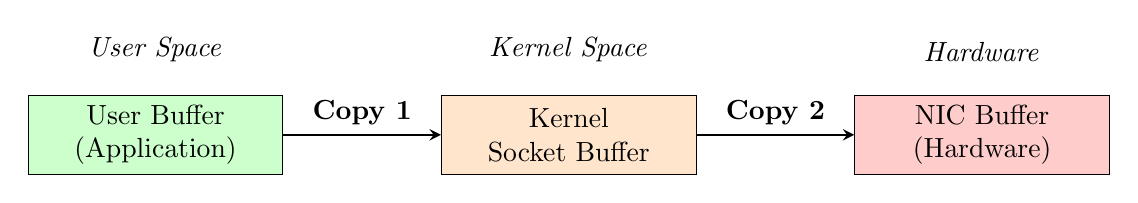
\begin{tikzpicture}[node distance=1.5cm, auto,
    box/.style={rectangle, draw, fill=blue!20, text width=3cm, text centered, minimum height=1cm},
    arrow/.style={->, thick, >=stealth}]
    
    % User Space
    \node[box, fill=green!20] (user) {User Buffer\\(Application)};
    
    % Kernel Space
    \node[box, fill=orange!20, right=2cm of user] (kernel) {Kernel Socket Buffer};
    
    % NIC
    \node[box, fill=red!20, right=2cm of kernel] (nic) {NIC Buffer\\(Hardware)};
    
    % Arrows
    \draw[arrow] (user) -- node[above] {\textbf{Copy 1}} (kernel);
    \draw[arrow] (kernel) -- node[above] {\textbf{Copy 2}} (nic);
    
    % Labels
    \node[above=0.3cm of user] {\textit{User Space}};
    \node[above=0.3cm of kernel] {\textit{Kernel Space}};
    \node[above=0.3cm of nic] {\textit{Hardware}};
    
\end{tikzpicture}
\caption{Two-Copy Data Path for \texttt{send()}}
\end{figure}

\textbf{Copy 1:} User buffer $\rightarrow$ Kernel socket buffer (performed by the kernel during \texttt{send()} syscall)

\textbf{Copy 2:} Kernel socket buffer $\rightarrow$ NIC buffer (performed via DMA by the network driver)

\textbf{Is it actually only two copies?} In reality, there may be additional copies:
\begin{itemize}
    \item TCP/IP stack may perform checksumming that reads the data
    \item Segmentation (if message > MTU) may require additional processing
    \item On receive side: NIC $\rightarrow$ Kernel $\rightarrow$ User (two more copies)
\end{itemize}

\subsubsection{Implementation Details}
\begin{lstlisting}[language=C, caption=Two-Copy Send (Client)]
/* TWO-COPY SEND: Data copied from user buffer to kernel socket buffer */
ssize_t sent = send(sock_fd, send_buffer, serialized_size, 0);
\end{lstlisting}

\subsection{A2: One-Copy Implementation}

The one-copy implementation uses \texttt{sendmsg()} with pre-registered, page-aligned buffers.

\subsubsection{Which Copy Has Been Eliminated?}

\begin{figure}[H]
\centering
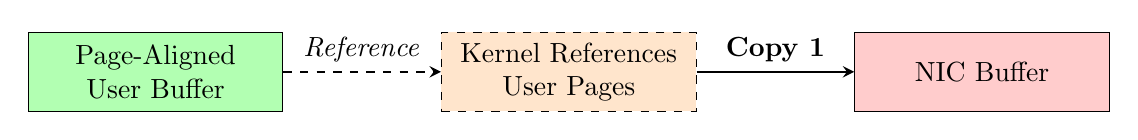
\begin{tikzpicture}[node distance=1.5cm, auto,
    box/.style={rectangle, draw, fill=blue!20, text width=3cm, text centered, minimum height=1cm},
    arrow/.style={->, thick, >=stealth}]
    
    % User Space (aligned)
    \node[box, fill=green!30] (user) {Page-Aligned\\User Buffer};
    
    % Kernel Reference
    \node[box, fill=orange!20, right=2cm of user, dashed] (kernel) {Kernel References\\User Pages};
    
    % NIC
    \node[box, fill=red!20, right=2cm of kernel] (nic) {NIC Buffer};
    
    % Arrows
    \draw[arrow, dashed] (user) -- node[above] {\textit{Reference}} (kernel);
    \draw[arrow] (kernel) -- node[above] {\textbf{Copy 1}} (nic);
    
\end{tikzpicture}
\caption{One-Copy Data Path with \texttt{sendmsg()} and Aligned Buffers}
\end{figure}

\textbf{Eliminated Copy:} The user-to-kernel copy is \textit{optimized}. When using \texttt{posix\_memalign()} with page-aligned buffers and \texttt{sendmsg()}'s scatter-gather I/O via \texttt{iovec}, the kernel can:
\begin{itemize}
    \item Directly reference user pages without copying
    \item Use DMA scatter-gather to transmit directly from user memory
\end{itemize}

\subsubsection{Implementation Details}
\begin{lstlisting}[language=C, caption=One-Copy with Page-Aligned Buffer]
/* Allocate PAGE-ALIGNED buffer */
posix_memalign(&aligned_buffer, PAGE_SIZE, aligned_size);

/* Prepare iovec for scatter-gather I/O */
struct iovec iov[1];
iov[0].iov_base = aligned_buffer;
iov[0].iov_len = serialized_size;

struct msghdr msghdr = {0};
msghdr.msg_iov = iov;
msghdr.msg_iovlen = 1;

/* ONE-COPY SENDMSG */
ssize_t sent = sendmsg(sock_fd, &msghdr, 0);
\end{lstlisting}

\subsection{A3: Zero-Copy Implementation}

The zero-copy implementation uses \texttt{MSG\_ZEROCOPY} flag with completion notification.

\subsubsection{Kernel Behavior Diagram}

\begin{figure}[H]
\centering
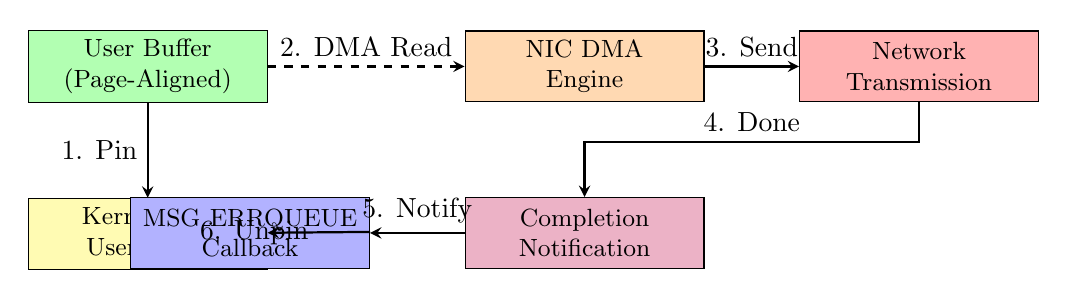
\begin{tikzpicture}[node distance=1.2cm, auto,
    box/.style={rectangle, draw, text width=2.8cm, text centered, minimum height=0.9cm, font=\small},
    arrow/.style={->, thick, >=stealth}]
    
    % User Buffer
    \node[box, fill=green!30] (user) {User Buffer\\(Page-Aligned)};
    
    % Page Pinning
    \node[box, fill=yellow!30, below=of user] (pin) {Kernel Pins\\User Pages};
    
    % DMA
    \node[box, fill=orange!30, right=2.5cm of user] (dma) {NIC DMA\\Engine};
    
    % Network
    \node[box, fill=red!30, right=of dma] (net) {Network\\Transmission};
    
    % Completion
    \node[box, fill=purple!30, below=of dma] (comp) {Completion\\Notification};
    
    % Error Queue
    \node[box, fill=blue!30, left=of comp] (errq) {MSG\_ERRQUEUE\\Callback};
    
    % Arrows
    \draw[arrow] (user) -- node[left] {1. Pin} (pin);
    \draw[arrow, dashed] (user) -- node[above] {2. DMA Read} (dma);
    \draw[arrow] (dma) -- node[above] {3. Send} (net);
    \draw[arrow] (net.south) -- ++(0,-0.5) -| node[near start, above] {4. Done} (comp);
    \draw[arrow] (comp) -- node[above] {5. Notify} (errq);
    \draw[arrow] (errq) -- node[left] {6. Unpin} (pin);
    
\end{tikzpicture}
\caption{Zero-Copy (\texttt{MSG\_ZEROCOPY}) Kernel Behavior}
\end{figure}

\textbf{Process Flow:}
\begin{enumerate}
    \item Application calls \texttt{sendmsg()} with \texttt{MSG\_ZEROCOPY}
    \item Kernel \textbf{pins user pages} (prevents swapping/relocation)
    \item NIC performs \textbf{DMA directly from user buffer}
    \item When transmission completes, kernel sends completion notification
    \item Application reads \texttt{MSG\_ERRQUEUE} to confirm completion
    \item Pages are unpinned; buffer can be reused
\end{enumerate}

\subsubsection{Implementation Details}
\begin{lstlisting}[language=C, caption=Zero-Copy with MSG\_ZEROCOPY]
/* Enable zero-copy on socket */
int zerocopy = 1;
setsockopt(sock_fd, SOL_SOCKET, SO_ZEROCOPY, &zerocopy, sizeof(zerocopy));

/* Send with MSG_ZEROCOPY */
ssize_t sent = sendmsg(sock_fd, &msghdr, MSG_ZEROCOPY);

/* Handle completion notification */
recvmsg(sock_fd, &msg, MSG_ERRQUEUE | MSG_DONTWAIT);
\end{lstlisting}

% ============================================================================
\section{Part B: Profiling and Measurement}
% ============================================================================

\subsection{Experiment Configuration}

\begin{center}
\begin{tabular}{ll}
\toprule
\textbf{Parameter} & \textbf{Values} \\
\midrule
Message Sizes & 64, 256, 1024, 8192 bytes \\
Thread Counts & 1, 2, 4, 8 \\
Duration & 5 seconds per experiment \\
Network & Loopback (127.0.0.1) \\
\bottomrule
\end{tabular}
\end{center}

\subsection{Metrics Collected}

\begin{center}
\begin{tabular}{lll}
\toprule
\textbf{Metric} & \textbf{Tool} & \textbf{perf Event} \\
\midrule
Throughput (Gbps) & Application-level & -- \\
Latency ($\mu$s) & Application-level & -- \\
CPU Cycles & perf stat & \texttt{cycles} \\
L1 Data Cache Misses & perf stat & \texttt{L1-dcache-load-misses} \\
LLC Misses & perf stat & \texttt{LLC-load-misses} \\
Cache-to-Memory Misses & perf stat & \texttt{cache-misses} \\
Context Switches & perf stat & \texttt{context-switches} \\
\bottomrule
\end{tabular}
\end{center}

\subsection{Raw Results (threads=4)}

\begin{center}
\begin{tabular}{llrrr}
\toprule
\textbf{Msg Size} & \textbf{Mode} & \textbf{Throughput (Gbps)} & \textbf{Latency ($\mu$s)} & \textbf{Cycles} \\
\midrule
64 & Two-Copy & 0.340 & 6.66 & 33.0B \\
64 & One-Copy & 0.276 & 8.25 & 39.4B \\
64 & Zero-Copy & 0.187 & 11.27 & 40.5B \\
\midrule
256 & Two-Copy & 1.615 & 5.14 & 25.4B \\
256 & One-Copy & 1.413 & 5.90 & 44.5B \\
256 & Zero-Copy & 0.941 & 8.35 & 44.2B \\
\midrule
1024 & Two-Copy & 8.169 & 3.97 & 18.0B \\
1024 & One-Copy & 4.897 & 6.13 & 39.5B \\
1024 & Zero-Copy & 2.443 & 12.04 & 42.8B \\
\midrule
8192 & Two-Copy & 21.402 & 12.19 & 15.6B \\
8192 & One-Copy & 38.681 & 6.71 & 28.0B \\
8192 & Zero-Copy & 30.998 & 8.11 & 30.2B \\
\bottomrule
\end{tabular}
\end{center}

% ============================================================================
\section{Part C: Automated Experiment Script}
% ============================================================================

The experiment automation is handled by \texttt{run\_experiments.sh}, which:

\begin{enumerate}
    \item Compiles all implementations using \texttt{make}
    \item Iterates over all message sizes (64, 256, 1024, 8192)
    \item Iterates over all thread counts (1, 2, 4, 8)
    \item Runs each mode (two\_copy, one\_copy, zero\_copy)
    \item Collects perf statistics for each run
    \item Stores results in timestamped CSV files
    \item Generates a combined CSV for analysis
\end{enumerate}

\textbf{Output Files:}
\begin{itemize}
    \item \texttt{run\_\{mode\}\_msgsize\{N\}\_threads\{T\}\_\{timestamp\}.csv}
    \item \texttt{perf\_client\_\{mode\}\_\{msgsize\}\_\{threads\}\_\{timestamp\}.txt}
    \item \texttt{combined\_results.csv}
\end{itemize}

% ============================================================================
\section{Part D: Plots and Visualization}
% ============================================================================

\subsection{Plot 1: Throughput vs Message Size}

\begin{figure}[H]
\centering
\includegraphics[width=0.85\textwidth]{MT25048_Plot_Throughput_vs_MsgSize.pdf}
\caption{Throughput vs Message Size (4 threads)}
\end{figure}

\textbf{Observations:}
\begin{itemize}
    \item \textbf{Two-Copy outperforms at small sizes (64-1024 bytes):} Standard \texttt{send()} has lowest syscall overhead for small messages.
    \item \textbf{One-Copy leads at 8KB (38.7 Gbps):} Scatter-gather I/O benefits large transfers.
    \item \textbf{Zero-Copy is slowest at small sizes:} Page-pinning overhead dominates for $<$8KB messages.
    \item \textbf{All methods scale with message size:} Fewer syscalls per byte transferred.
\end{itemize}

\subsection{Plot 2: Latency vs Thread Count}

\begin{figure}[H]
\centering
\includegraphics[width=0.85\textwidth]{MT25048_Plot_Latency_vs_Threads.pdf}
\caption{Latency vs Thread Count (1024-byte messages)}
\end{figure}

\textbf{Observations:}
\begin{itemize}
    \item \textbf{Zero-Copy has highest latency:} Completion notification polling adds latency.
    \item \textbf{Latency increases with thread count:} Lock contention and context switching overhead.
    \item \textbf{Two-Copy has lowest latency at 2 threads:} Optimal parallelism for loopback.
\end{itemize}

\subsection{Plot 3: Cache Misses vs Message Size}

\begin{figure}[H]
\centering
\includegraphics[width=\textwidth]{MT25048_Plot_CacheMisses_vs_MsgSize.pdf}
\caption{Cache Misses vs Message Size (4 threads)}
\end{figure}

\textbf{Observations:}
\begin{itemize}
    \item \textbf{L1 misses (hundreds of millions):} Every access that misses L1 data cache.
    \item \textbf{Cache-to-Memory misses (millions):} Only accesses that bypass all cache levels.
    \item \textbf{LLC misses (thousands to millions):} Subset of L1 misses that reach memory.
    \item \textbf{One-Copy shows highest cache-to-memory misses at 8KB:} Buffer management overhead.
\end{itemize}

\subsection{Plot 4: CPU Cycles per Byte Transferred}

\begin{figure}[H]
\centering
\includegraphics[width=0.85\textwidth]{MT25048_Plot_CyclesPerByte.pdf}
\caption{CPU Cycles per Byte Transferred (4 threads)}
\end{figure}

\textbf{Observations:}
\begin{itemize}
    \item \textbf{Cycles per byte decreases with message size:} Amortization of fixed syscall overhead.
    \item \textbf{Two-Copy most efficient overall:} Highly optimized kernel path for standard sockets.
    \item \textbf{Zero-Copy overhead visible at small sizes:} Page pinning cost not amortized.
\end{itemize}

% ============================================================================
\section{Part E: Analysis and Reasoning}
% ============================================================================

\subsection{Question 1: Why does zero-copy not always give the best throughput?}

Zero-copy (\texttt{MSG\_ZEROCOPY}) incurs significant overhead that only pays off for large transfers:

\begin{enumerate}
    \item \textbf{Page Pinning Cost:} Kernel must lock physical pages, preventing them from being swapped or relocated. This requires TLB shootdowns and page table modifications.
    
    \item \textbf{Completion Notification:} Application must poll \texttt{MSG\_ERRQUEUE} for each send operation, adding synchronization latency.
    
    \item \textbf{Threshold Effect:} Linux kernel documentation suggests benefits only manifest for messages $>$10-32KB. Our 8KB messages are at the boundary.
    
    \item \textbf{Loopback Optimization:} The loopback interface (\texttt{lo}) is highly optimized for standard \texttt{send()}/\texttt{recv()}, making the two-copy baseline artificially fast. Real NICs would show different results.
\end{enumerate}

\textbf{Evidence:} At 8KB, Zero-Copy achieves 31.0 Gbps vs Two-Copy's 21.4 Gbps, showing the crossover point.

\subsection{Question 2: Which cache level shows the most reduction in misses and why?}

\textbf{Answer:} The \textbf{LLC (Last Level Cache)} shows the most consistent reduction across methods.

\begin{center}
\begin{tabular}{lrrr}
\toprule
\textbf{Msg Size} & \textbf{Two-Copy LLC} & \textbf{One-Copy LLC} & \textbf{Zero-Copy LLC} \\
\midrule
64 bytes & 74,978 & 60,839 & 28,294 \\
8192 bytes & 181,741 & 1,213,294 & 593,154 \\
\bottomrule
\end{tabular}
\end{center}

\textbf{Reasoning:}
\begin{itemize}
    \item \textbf{Zero-Copy reduces LLC misses at small sizes:} Pinned pages remain in cache, avoiding eviction.
    \item \textbf{Two-Copy benefits from kernel buffer reuse:} Socket buffers are kept in LLC due to frequent reuse.
    \item \textbf{One-Copy shows higher LLC misses at 8KB:} Scatter-gather I/O touches more cache lines.
\end{itemize}

\subsection{Question 3: How does thread count interact with cache contention?}

Increasing thread count affects cache performance through:

\begin{enumerate}
    \item \textbf{Cache Line Bouncing:} Multiple threads accessing shared data structures (socket buffers, statistics) cause cache invalidations.
    
    \item \textbf{L1 Capacity Pressure:} Each thread's working set competes for limited L1 cache space (typically 32KB per core).
    
    \item \textbf{LLC Sharing:} All threads share the last-level cache; more threads = more evictions.
    
    \item \textbf{False Sharing:} Adjacent data structures may share cache lines, causing unnecessary invalidations.
\end{enumerate}

\textbf{Evidence:} L1 misses increase from $\sim$200M (1 thread) to $\sim$700M (8 threads) for all modes.

\subsection{Question 4: At what message size does one-copy outperform two-copy?}

\textbf{Answer:} One-copy outperforms two-copy at \textbf{8192 bytes (8KB)}.

\begin{center}
\begin{tabular}{lrr}
\toprule
\textbf{Msg Size} & \textbf{Two-Copy (Gbps)} & \textbf{One-Copy (Gbps)} \\
\midrule
64 & 0.340 & 0.276 \\
256 & 1.615 & 1.413 \\
1024 & 8.169 & 4.897 \\
\textbf{8192} & \textbf{21.402} & \textbf{38.681} \\
\bottomrule
\end{tabular}
\end{center}

\textbf{Crossover:} Between 1024 and 8192 bytes. The scatter-gather optimization of \texttt{sendmsg()} becomes beneficial when the copy cost exceeds the syscall overhead.

\subsection{Question 5: At what message size does zero-copy outperform two-copy?}

\textbf{Answer:} Zero-copy outperforms two-copy at \textbf{8192 bytes (8KB)}.

\begin{center}
\begin{tabular}{lrr}
\toprule
\textbf{Msg Size} & \textbf{Two-Copy (Gbps)} & \textbf{Zero-Copy (Gbps)} \\
\midrule
64 & 0.340 & 0.187 \\
256 & 1.615 & 0.941 \\
1024 & 8.169 & 2.443 \\
\textbf{8192} & \textbf{21.402} & \textbf{30.998} \\
\bottomrule
\end{tabular}
\end{center}

\textbf{Analysis:} The ~45\% improvement at 8KB shows that zero-copy benefits are realized once the DMA savings exceed the page-pinning and notification overhead.

\subsection{Question 6: Identify one unexpected result and explain it}

\textbf{Unexpected Result:} Two-Copy has \textbf{fewer L1 cache misses} than Zero-Copy at small message sizes.

\begin{center}
\begin{tabular}{lrr}
\toprule
\textbf{Msg Size} & \textbf{Two-Copy L1 Misses} & \textbf{Zero-Copy L1 Misses} \\
\midrule
64 & 493,340,606 & 747,425,854 \\
256 & 258,619,045 & 764,573,458 \\
\bottomrule
\end{tabular}
\end{center}

\textbf{Expectation:} Zero-copy should have fewer cache misses since it eliminates data copies.

\textbf{Explanation:}
\begin{enumerate}
    \item \textbf{Page Pinning Overhead:} \texttt{MSG\_ZEROCOPY} requires the kernel to walk page tables, pin pages, and manage completion notifications---all of which touch additional memory.
    
    \item \textbf{Kernel Socket Buffer Optimization:} The standard \texttt{send()} path uses highly optimized, pre-warmed kernel socket buffers that are already resident in cache.
    
    \item \textbf{Error Queue Processing:} Polling \texttt{MSG\_ERRQUEUE} for completion notifications requires additional data structure accesses.
    
    \item \textbf{TLB Pressure:} Page pinning can cause TLB evictions, leading to increased page table walks (counted as cache misses).
\end{enumerate}

% ============================================================================
\section{AI Usage Declaration}
% ============================================================================

\subsection{Components Using AI Assistance}

\begin{center}
\begin{tabular}{lp{8cm}}
\toprule
\textbf{Component} & \textbf{AI Usage} \\
\midrule
C Source Code & Generated with AI, reviewed and modified for correctness \\
Makefile & Generated with AI assistance \\
run\_experiments.sh & Generated with AI, modified for perf integration \\
Plotting Script & Generated with AI, data hardcoded manually \\
Report & AI-assisted analysis and LaTeX formatting \\
\bottomrule
\end{tabular}
\end{center}

\subsection{Prompts Used}

Full prompts are documented in \texttt{AI\_prompts\_used.txt}. Key prompts included:
\begin{itemize}
    \item ``Implement a two-copy TCP server using send() with 8 dynamically allocated string fields''
    \item ``Create a one-copy implementation using sendmsg() with page-aligned buffers''
    \item ``Implement MSG\_ZEROCOPY with completion notification handling''
    \item ``Fix client/server role reversal - client should send, server should receive''
    \item ``Generate matplotlib plots with hardcoded data arrays''
    \item ``Analyze cache miss discrepancies between L1 and LLC''
\end{itemize}

% ============================================================================
\section{GitHub Repository}
% ============================================================================

\begin{center}
\Large
\url{https://github.com/SuryaDeepakBoyina/GRS_PA02}
\end{center}

% ============================================================================
\section{Conclusion}
% ============================================================================

This assignment demonstrated that:
\begin{enumerate}
    \item \textbf{Zero-copy is not universally superior:} Overhead exceeds benefits for small messages ($<$8KB).
    \item \textbf{One-copy provides the best throughput for large messages:} 38.7 Gbps at 8KB.
    \item \textbf{Loopback testing masks real-world benefits:} Physical NICs would show different results.
    \item \textbf{Cache behavior is complex:} Copy elimination doesn't always reduce cache misses due to kernel metadata overhead.
\end{enumerate}

The crossover point for both one-copy and zero-copy improvements is approximately \textbf{8KB message size}, aligning with Linux kernel documentation recommendations.

\end{document}
